\documentclass[a4paper,UKenglish]{lipics}
%This is a template for producing LIPIcs articles. 
%See lipics-manual.pdf for further information.
%for A4 paper format use option "a4paper", for US-letter use option "letterpaper"
%for british hyphenation rules use option "UKenglish", for american hyphenation rules use option "USenglish"
% for section-numbered lemmas etc., use "numberwithinsect"
 
\usepackage{microtype}%if unwanted, comment out or use option "draft"

%\graphicspath{{./graphics/}}%helpful if your graphic files are in another directory

\bibliographystyle{plain}% the recommended bibstyle

% Author macros::begin %%%%%%%%%%%%%%%%%%%%%%%%%%%%%%%%%%%%%%%%%%%%%%%%
\title{A Diagnostic Approach for Static Program Analysis}
\titlerunning{Diagnostic Analysis} %optional, in case that the title is too long; the running title should fit into the top page column

\author{}
%\author[2]{Joan R. Access}
%\affil[1]{Dummy University Computing Laboratory\\
%  Address, Country\\
%  \texttt{open@dummyuni.org}}
%\affil[2]{Department of Informatics, Dummy College\\
%  Address, Country\\
%  \texttt{access@dummycollege.org}}
%\authorrunning{J.\,Q. Open and J.\,R. Access} %mandatory. First: Use abbreviated first/middle names. Second (only in severe cases): Use first author plus 'et. al.'

%\Copyright{John Q. Open and Joan R. Access}%mandatory, please use full first names. LIPIcs license is "CC-BY";  http://creativecommons.org/licenses/by/3.0/

%\subjclass{Dummy classification -- please refer to \url{http://www.acm.org/about/class/ccs98-html}}% mandatory: Please choose ACM 1998 classifications from http://www.acm.org/about/class/ccs98-html . E.g., cite as "F.1.1 Models of Computation". 
\keywords{JavaScript, points-to analysis, debugging}% mandatory: Please provide 1-5 keywords
% Author macros::end %%%%%%%%%%%%%%%%%%%%%%%%%%%%%%%%%%%%%%%%%%%%%%%%%

%Editor-only macros:: begin (do not touch as author)%%%%%%%%%%%%%%%%%%%%%%%%%%%%%%%%%%
%\serieslogo{}%please provide filename (without suffix)
%\volumeinfo%(easychair interface)
%  {Billy Editor and Bill Editors}% editors
%  {2}% number of editors: 1, 2, ....
%  {Conference title on which this volume is based on}% event
%  {1}% volume
 % {1}% issue
 % {1}% starting page number
%\EventShortName{}
%\DOI{10.4230/LIPIcs.xxx.yyy.p}% to be completed by the volume editor
% Editor-only macros::end %%%%%%%%%%%%%%%%%%%%%%%%%%%%%%%%%%%%%%%%%%%%%%%

\begin{document}

\maketitle

\begin{abstract}

 \end{abstract}

\section{Introduction}

\section{Motivation \& Background}

\subsection{Motivating Example}
In this section, we would like to use a code example (or a series of examples; see below) to demonstrate the difficulties to (manually) find the performance bottleneck of a static analysis. For example, Figure \ref{fig:jquery-orig} shows the original {\tt extend} function of jQuery whose behavior is not easy to understand; moreover, due to its usage of complicated program structures (e.g., recursion, function variadicity), it is difficult for an analysis to accurately model the results of this function (confirmed in \cite{}). In \cite{}, the authors had to manually transform this function to simplify its structure, resulting in the code in Figure \ref{fig:jquery-modified}. Nevertheless, the transformed code, in and of itself, is still insufficient for a field-sensitive analysis to complete analyzing simple jQuery applications. Therefore, the authors of \cite{} designed an automatic function extraction algorithm (correlation extraction) and used argument sensitivity to improve the performance and precision of JavaScript points-to analysis. The code that is actually being analyzed by the argument-sensitive analysis is presented in Figure \ref{fig:jquery-extracted}. Overall, the take-away message shall be: it is difficult to locate the analysis bottleneck and it is also difficult to find a solution to improve the analysis. This series of examples strongly support the above statement: (1) among almost 9,000 lines of code of jQuery library, it usually is clueless to know that one particular function results in the analysis performance bottleneck (without investigating the code); (2) even if the analysis designer is able to locate this function as the bottleneck, it is difficult to tell which program structure or if it is the combination of several program structures that result in bad analysis behavior, thus making it difficult to develop new technology to improve the analysis; (3) even if the analysis designer is able to (manually) abstract away several challenges (e.g., the transformed function in Figure \ref{fig:jquery-modified}), and wants to apply the more precise technique whole program (e.g., argument sensitivity), this may in turn results in overhead because the other portion of the program may not benefit from the more advanced technique (although this particular function will significantly benefit from argument sensitivity). ({\bf Comment from Shiyi: despite that I think this is a good series examples as motivation, we cannot afford to use too much space for the codes; simplify the code, especially Figure 1 (included the complete code for your reference), as the ECOOP 12 paper did; or use one whole example to demonstrate what we want to express. Also, note that our technique does not automatically fixes the issues discussed in (1) and (2) above, while we do locate the bottleneck function and apply the advanced techniques, thus solving problem (3) above.}).

\begin{figure}[th!]
        \lstinputlisting{jquery-orig.js}
\caption{\textmd{Original {\tt extend} function of jQuery 1.6.1.}}
\label{fig:jquery-orig}
\end{figure}

\begin{figure}[th!]
        \lstinputlisting{jquery-modified.js}
\caption{\textmd{Modifed {\tt extend} function of jQuery 1.6.1.}}
\label{fig:jquery-modified}
\end{figure}

\begin{figure}[th!]
        \lstinputlisting{jquery-extracted.js}
\caption{\textmd{Mofified {\tt extend} function with correlation extraction \cite{} of jQuery 1.6.1}}
\label{fig:jquery-extracted}
\end{figure}

\subsection{Static Points-to Analysis Behavior (Empirical Study)}
To (manually or automatically) understand and debug the performance and precision issues associated with static points-to analysis, it is important to know its behavior (normal and abnormal). We present some data to characterize the points-to analysis behavior.

1. growth of points-to graph size (points-to edges) during points-to analysis lifetime. Figure \ref{fig:pts-growth} shows the growth rate of two points-to analyses on an application that invokes jQuery 1.6.1 library. The bad points-to analysis is the baseline analysis (i.e., 0-1-cfa) which could not finish under limited time budget (10 minutes); the good points-to analysis is a 1-cfa and argument-sensitive which finishes analyzing the program in less than 5 seconds and the total number of points-to iteration is about 118,000. Comparing the life time of the bad (part of its lifetime as its lifetime could be much longer) and the good points-to analysis, we observe the growth rate of points-to size (i.e., we count the total number of points-to edges in the graph every 5000 iterations) of good points-to analysis is steady while the bad points-to analysis has ``jumps" (indicating the approximation and "pollution" of points-to results). This finding motivated us to design heuristics to decide when we would like to perform the automatic diagnostic analysis for a bad analysis (i.e., when the slope of growth significantly change). ({\bf Comment by Shiyi: the data of Figure \ref{fig:pts-growth} is included in section2-results.xlsx. I think this is interesting and we may need one more figure on other programs to better support our argument.})

\begin{figure}[th!]
        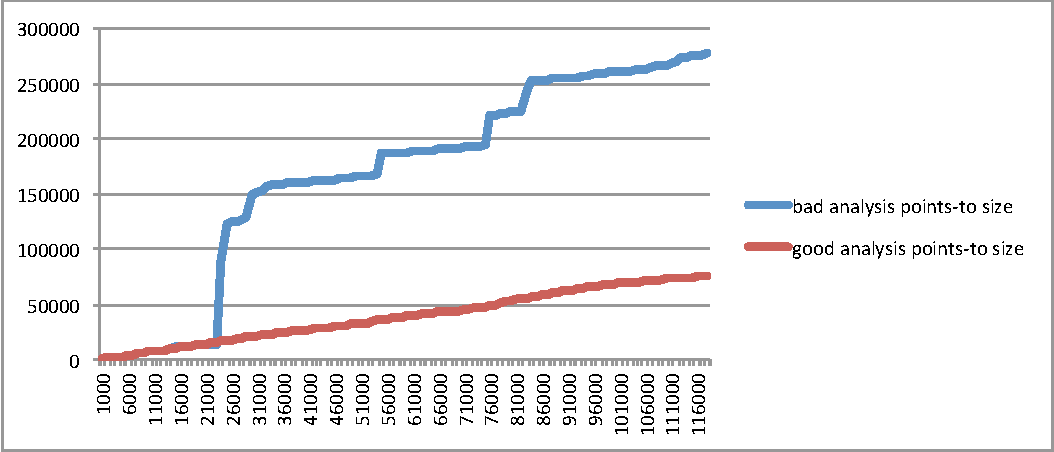
\includegraphics[width=0.95\columnwidth]{pts-growth}
\caption{\textmd{Characteristics of points-to size growth.}}
\label{fig:pts-growth}
\end{figure}

2. Points-to size (per pointer key) distribution. See section2-results.xlsx for the data (columns I and J). The data show very interesting and different characteristics of points-to size distribution between a good and bad points-to analyses (the same analyses as in Figure \ref{fig:pts-growth}). We collected this data for each analysis after 100,000 iterations. I think we are looking for a frequency graph here that x axis represents the size of points-to size and y axis represents the number of pointer keys with the specific size of points-to set. Roughly looking at the data, for example in column I (the good points-to analysis), the curve is likely to evenly going down with the increase of points-to size. While for the bad points-to analysis (column J), the curve seems evenly going down with the increase of points-to size until the size of 33; after 33, the next size jumps to 150, and there are a lot of pointer keys with points-to size greater than 150 (thus, the frequency graph/curve/histogram would grow after specific number for the bad analysis). This result is interesting in that this indicates for a bad points-to analysis, some approximate results polluted a lot of places in the graph; thus making the analysis unscalable and extremely imprecise. ({\bf Comment by Shiyi: I can use excel to generate the frequency graph, but it may take some time for me to do so, but I do think this result is interesting to report because the "outliers" (i.e., many pointer keys with large points-to size) in the bad points-to graph indicate how the bottleneck can pollute the analysis and that motivates us find the bottleneck. Furthermore, taking close look at the "large" points-to sizes, many pointer keys share the same points-to sizes, indicating that many could be copies from previously approximate results; thus being "polluted" after copying. This finding motivates us to track the copies of points-to sets during the diagnosis.})

3... We may think of more to report on points-to analysis characteristics. We shall focus on the characteristics that distinguish the good and bad points-to analysis. More data make this subsection an empirical study of static points-to analysis behavior and characterization of good/bad points-to analysis, which in and of itself is a good effort and something new to present, thus making it a contribution of this paper.

({\bf Further comments on Section 2 by Shiyi: I think with the empirical study, this section can be long, but it is Ok as we already are presenting new observations and findings in this section. These new findings very well serve the motivation and design guidance of our algorithm; thus very tightly connected to the rest of the paper.})

\section{Overview \& Design}

\section{Implementation}

\section{Evaluation}

\section{Related Work}

\section{Conclusions}

\end{document}
